\chapter{Implementation}
In this chapter it is described in details the framework that it has been implemented for assess the SQL-compliance for current DBMSs.

\section{Implementation}
The architecture composes by three different tools as their were introduced in the methodology chapter. The first two tools are implemented in Java programming language and the other one is implemented in python programming language which it is an open source project that can generate random realistic data.  It is chosen Java programming language since it is very popular and it can be used to build cross-platform systems. The complete architecture consists by twenty java classes. 

 \begin{figure} 
      \centering
      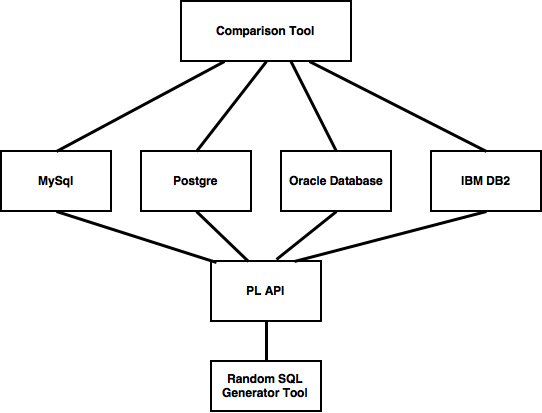
\includegraphics[width=\textwidth,height=6cm]{Images/1-implemen_detail}
      \caption{Random SQL Generator Architecture}
      \label{fig:counting-methods}
  \end{figure}

\subsection{Random SQL generator engine}
An important component of the architecture is the random SQL generator tool which is used to generate random SQL queries for assessing modern DBMSs. SQL language consists by numerous SQL commands and therefore some of them are simple in terms of their usage such as SELECT, FROM, WHERE where some others are more trickier such as GROUP BY, HAVING or aggregation functions where it is needed to be cared about the proper use of these commands and generating syntactically correct SQL queries. As a result, for achieving generating meaningful and syntactically valid queries, the current implementation of generator tool composes by various java classes specifically seventeen classes, and each class is used for generating different SQL Clause. 

In addition, the tool has been designed in such a way that it is modular and reusable and therefore new systems can easily added without the need of changing the whole structure of the tool.

An important decision which should be taken it was with regards to the internal generator tool in order to make it feasible to generate different valid SQL queries and simultaneously syntactically correct. Hence, it is implemented an internal representation and each class is responsible for generating a different SQL clauses that contribute to the overall query. For example, one of the java classes generate the SELECT clause. Having different classes for each SQL statement, it makes it easier to extend the tool in order to add new functionality and at the same time there is no need to change other part of the tool. The final SQL query is converted to an SQL string which then is executed to the current DBMSs with the contribution of the comparison tool. An important note is that it is not feasible to generate SQL strings directly because it is needed to track attributes names and types. If it was being generated just strings, it would not possible to check if in the WHERE clause it is mentioning attributes that appear in the FROM clause or they comes as parameters from the outer query. Thusly, there is a need to track attributes for each clause and to achieve that they have been used to main data structure such as LinkedList and HashMaps.

\subsection{Configuration file}
The generator tool consists also by a configuration file for partially control the random SQL queries and a detailed explanation is given as follow: The configuration file is used to provide information to the generator tool. Therefore, many parameters can be specified from the configuration file. Below, it is provided firstly the format of the configuration file and subsequently a comprehensive explanation is given  for every parameter. 

\begin{mdframed}[backgroundcolor=gray!20] 
  This configuration file will be used to give various parameter
  \\ to the SQLEngine

  Maximum number of tables in the FROM STATEMENT
\\maxTablesFrom =3

  Maximum number of attributes in the SELECT STATEMENT
\\maxAttrSel =5

  Maximun number of comparisons in the WHERE STATEMENT
\\maxCondWhere =7

 Represents the probability of having constants or NULL comparison \\ in the WHERE STATEMENT
\\probWhrConst = 0.8

 nestLevel = 4
\end{mdframed}

Another important decision that should be taken into account is how we can provide the relations and attributes to the tool. An initial approach was to be given as parameters in the configuration file. Albeit this approach works pretty well, it makes our tool not portable. Image if the DBMSs have lots of tables with many columns. Hence, It will be time-consuming to give these parameters via the configuration files. Thus, an efficient approach is to retrieve the whole schema from DBMSs automatically. As a result, our tool has the capability to automatically retrieve the whole schema for any DBMS just by providing the credential for connecting to the database in the configuration file.   

All the parameters are described as follow:
\begin{description}
   \item[$\bullet$ relations and attributes] =  parameters are used to provide to the generator tool the tables and columns for generating SQL queries according to the database schema. Albeit this approach works pretty well, it makes our tool not portable. Image if the DBMS has a large number of tables with many columns. Hence, the current architecture had the capability to automatically retrieve the whole database schema from DBMSs by just providing the credential in the configuration file by configure user, pass and dbName parameters. 

\item[$\bullet$ MaxTablesFrom] = parameter is used to set an upper bound of the number of tables that an FROM clause can have. If the upper bound is greater than the total number of tables in the schema, then the upper bound is automatically defines the the total number of tables. 

\item[$\bullet$ MaxAttrSel] = parameter indicates an upper bound of projections that the Select clause can have. In other words, it is the total number of attributes that can be selected in the Select clause.
 
\item[$\bullet$ MaxCondWhere]= parameter represents the total number of comparison that the Where clause can have. 

 
\item[$\bullet$ ProbWhrConst] = parameter represents the probability of having comparisons with constant or Null in the Where clause. Therefore, a number between 0 and 1 can be given for this parameter.  

\item[$\bullet$ RepAlias]= parameter indicates the probability of having repetition of alias in the Select clause. 

\item[$\bullet$ NestLevel]= parameter represents the maximum level of nesting that a query can have. For generating such a query many consideration should be taken into account. For example, we should track attributes for outer queries, as inner query can access outer attributes or attributes from its FROM clause. The opposite is not true, meaning that we cannot access attributes from an inner query. 

\item[$\bullet$ ArithCompSel] = parameter represents the probability of having arithmetic operations in the Select clause. 

\item[$\bullet$ Dinstinct ] = parameter represents the probability of appearing the distinct SQL statement in a query. 

\item[$\bullet$ StringInSel] = parameter indicates the probability of projecting an attribute of type string or having string functions. 

\item[$\bullet$ StringInWhere] = parameter represents the probability of having string comparison in Where clause. 
\end{description} 

As a consequence, our tool supports a configuration file that can be used to control the randomly generated SQL queries. Below is provided a part of the configuration file and some of the main parameters are explained

It can be seen from the configuration file that we can control many parameters, nevertheless it does not imply that we restrict the diversity of SQL query that can be generated. For example, we can set an upper bound of tables that appear in the FROM clause. In that way, we avoid having an enormous table size from cartesian product. In addition, even it is not so usual to have constant comparison in an SQL query, nevertheless SQL standards support this. Thus, we generate SQL queries which have constant comparisons but we do not need to have a lot of such queries. An example of such query is as follow:

\begin{mdframed}[backgroundcolor=gray!20] 
SELECT r41.A AS A0
\\FROM r4 AS r41
\\WHERE 1 > 2
\end{mdframed}

There are plenty of SQL commands that can be used to manipulate the data. Below we summarize all the SQL commands which our random query generator use to generate SQL queries.   


\section{Comparison Tool} 
As it was mentioned, the overall objective of the implemented architecture is to be capable of detecting  any difference that may exist among current systems. For accomplishing that, aside from the random SQL generator tool,  the comparison tool (CT) is implemented as well. Each random SQL query should be executed on five systems. As a consequence, the whole process should be automated and differences that may arise should be documented into a log file. Below, it is illustrated the comparison tool (CT) which has been implemented for achieving the aforementioned purposes and further it is provided a detailed explanation of the internal implementation of the tool.  


 \begin{figure} 
      \centering
      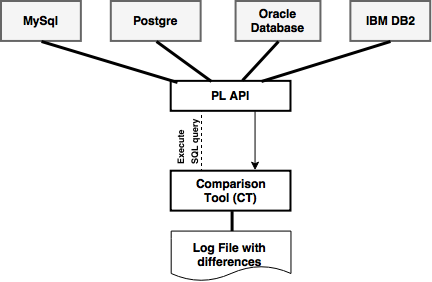
\includegraphics[width=\textwidth,height=6cm]{Images/2-ComparisonTool}
      \caption{Simple Architecture of Comparison Tool}
      \label{fig:counting-methods}
  \end{figure}

It has been implemented in Java programming language in order to compare the result of each query on each DBMSs. The CT is fully compatible with the random generator engine and it takes as input each SQL query which is generated by the random SQL generator and subsequently evaluates each query to all the DBMSs. For comparing the results, some challenges had to be overcome. For instance, each DBMS use different algorithms to evaluate each query and it returns the rows of the result in different order or situations with various format. For overcoming  the problem of different rows’ ordering, it is used a data structure such as LinkedList to store the result and then an efficient in-memory sorting algorithm is performed to sort the result. Apparently now, it is expected all the result among the DBMSs to be identical and therefore they can be compared. In the event of a difference is found or a query raises an error, it is documented in the log file. More precisely, the log file contains the SQL query that causes the problem and the exact systems that the difference is found. In addition, if a system raises an error without even to be possible to execute the query, the specific error is recorded with the associated system that raises the error. An important consideration for implementing this tool is how to implementing in a way that in the future new systems can be efficiently added. 

As a result, the core idea behind this, it is that there is one method that executes each query and compares the results for any DBMS. Thus, this method takes the connection for accessing the systems and retrieve the result. In the future, if a new DBMS need to be checked can be easily added by providing the connection to this method without changing the internal state of the method.  
 It is illustrated in the experiments chapter  that indeed differences exist and in some situations may be significant depends on the context that the queries are used. Also, the tool is an important component of this project as it is used to conduct the experiments and identify the main differences that exist between current DBMSs. 

 \begin{figure} 
      \centering
      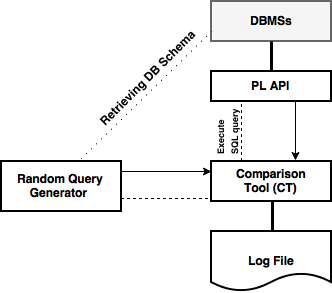
\includegraphics[width=\textwidth,height=6cm]{Images/3-ComparisonTool}
      \caption{Architecture of Comparison Tool}
      \label{fig:counting-methods}
  \end{figure}

\section{Generate data}
Datafiller is a well-known open-source project that provides the capability of generating random data. For our project data filler is very important as it will be used for generating a diversity of  data sets in order to evaluate all major DBMSs. More precisely, the datafiller script generates random data, based on a data schema which is provided as a parameter, and it takes into account constraints of that schema for generating valid data. For example, it takes into account the domain of each field and if the field should be unique, foreign key or primary key. Another important parameter is the df: null=rate% which indicated nullable rates. It will be extremely useful to test the behaviour of current DBMS in a database with nulls and check if there are differences.     

Additionally, more complex parameters can be provided as well, such as the number of tuples per table using --size SIZE parameter. It worthy mentioning that these parameters should be defined within the schema script and should start with -- df.  Further, we can generate more realistic data by providing some information in schema SQL script. For instance, if there is a field which represents a date, then we can provide a range in order for the datafiller to generate dates only within that range. This can be achieved by specifying the following parameter: range -- df: start=year-month-day end=year-month-day beside the date field. Subsequently, we need to add the --filter parameter while running the script. These are only some of the important parameters that the datafiller provides but apart from these, it provides more sophisticated properties which are out of importance for our project.


 \begin{figure} 
      \centering
      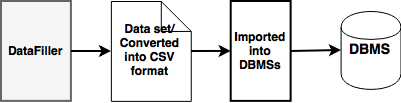
\includegraphics[width=\textwidth,height=2cm]{Images/4-Datafiller}
      \caption{Method of importing csv files}
      \label{fig:counting-methods}
  \end{figure}  


Datafiller supports data importing only into PostgreSQL. Nevertheless, for our project we need to import the random generated data into five DBMSs. For this reason, we convert the data into CSV format, as all of them support importing data from CSV files.  

